\section{Tabelle riassuntive}

\subsection{Ordinamento}

\begin{figure}[h]
    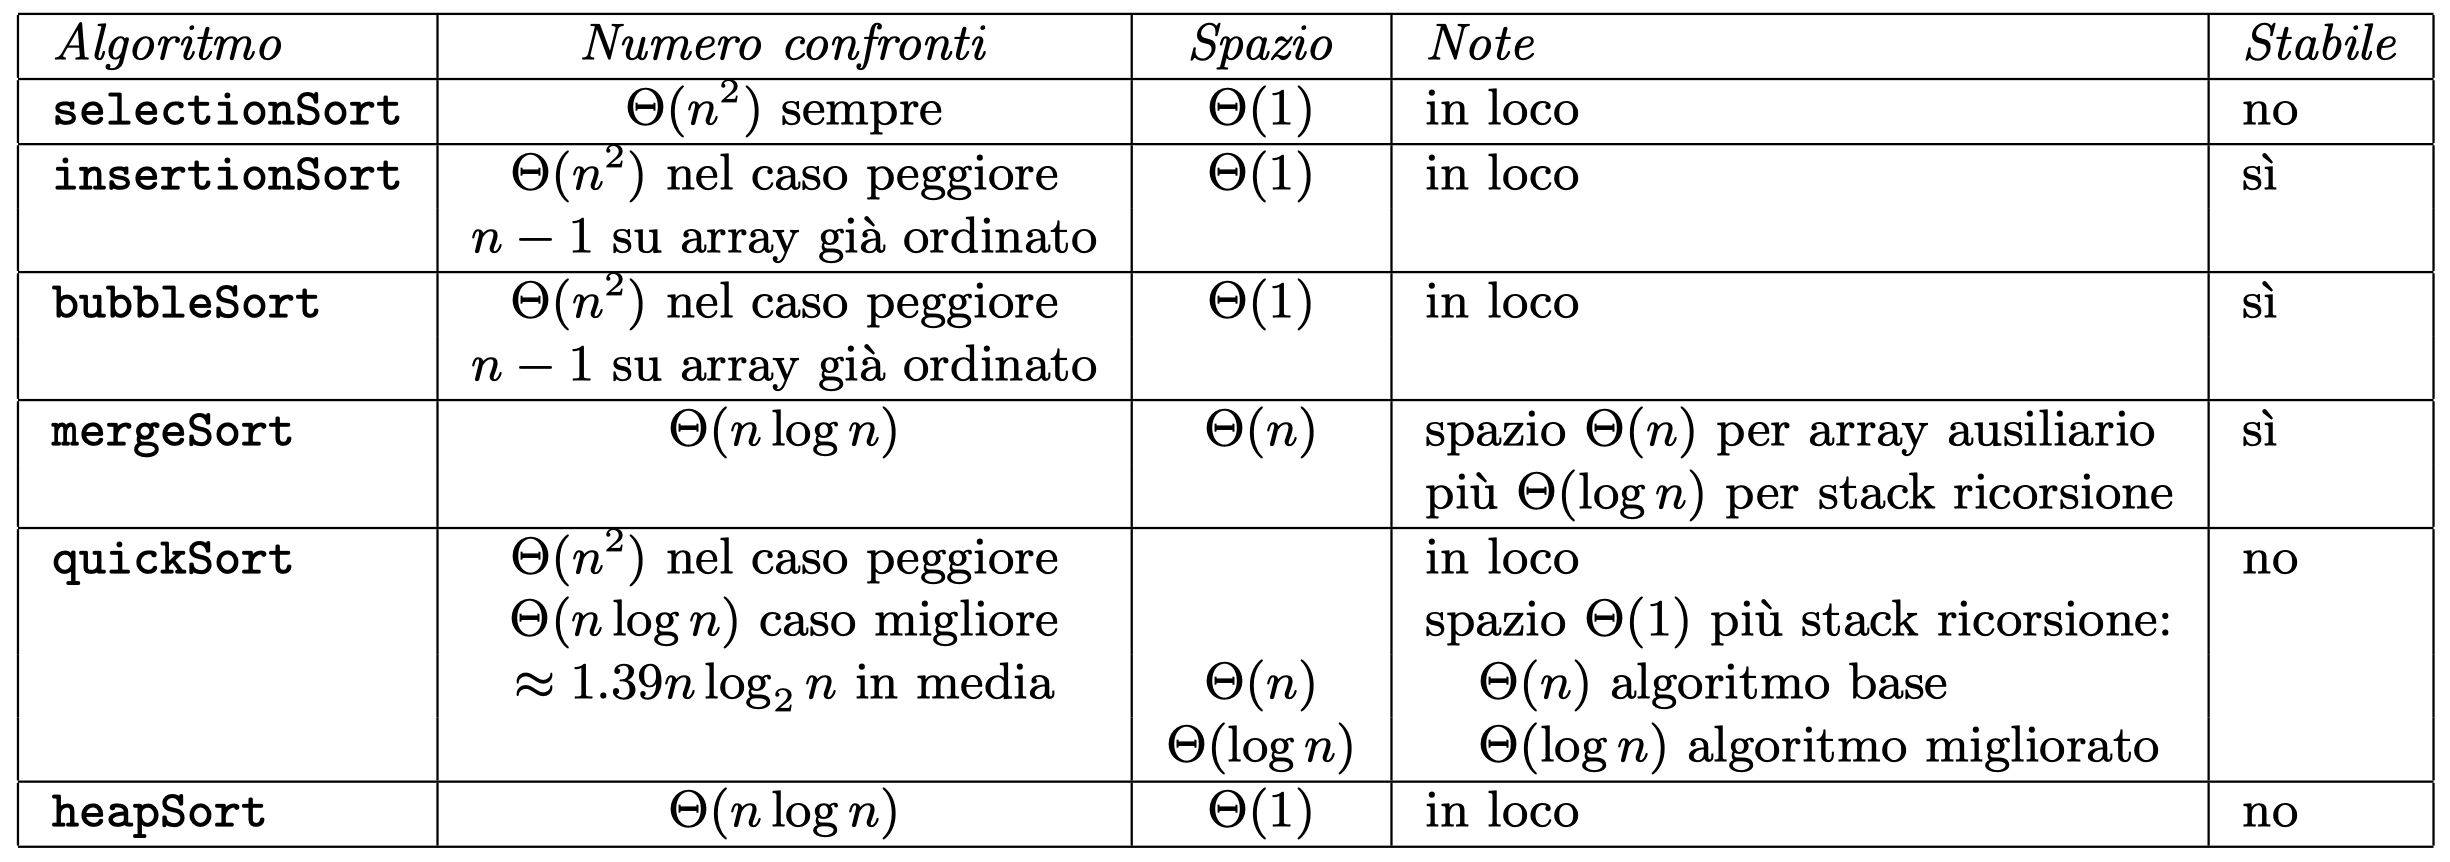
\includegraphics[width=\textwidth]{riepilogo_ordinamento.png}
\end{figure}

\subsection{Complessità temporale strutture dati}
\begin{figure}[h]
    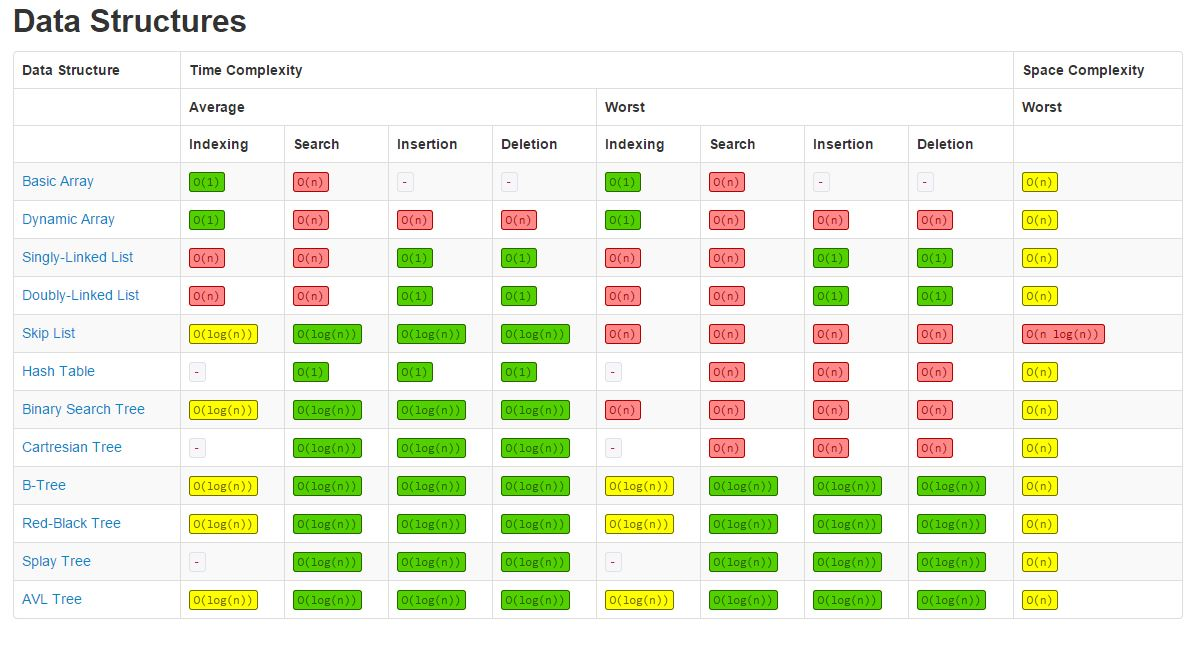
\includegraphics[width=\textwidth]{dscomplexity.png}
\end{figure}


\subsection{Alberi: numero di nodi e altezza}

\begin{tabular}{|l|c|c|}
    \hline
    \textbf{Struttura} & \textbf{Numero di nodi} & \textbf{Altezza}\\
    \hline
    \textbf{Alberi binari di ricerca} & $h + 1 \le n \le 2^{h+1}-1$ & $\log_2(n+1) - 1 \le h \le n - 1$\\
    \hline
    \textbf{Alberi 2-3} & $2^{h+1}-1 \le n \le \frac{3^{h+1}-1}{2}$ & \space \\
    \hline
    \textbf{B-alberi} & $\ge 2t^h -1$ & \space\\
    \hline
    \textbf{Heap} & $2^h \le n \le 2^{h + 1}$ & $h \le \log_2 n \le h + 1$\\
    \hline
\end{tabular}